\documentclass{acm_proc_article-sp}
\usepackage[linesnumbered]{algorithm2e}
\usepackage{float}
\usepackage{qtree}

%%% Header
\title{Facilitating Large-Scale Graph Search Algorithms with Lock-Free Concurrent Pairing Heaps}

\numberofauthors{3}

\author{
\alignauthor
Jeremy Mayeres \\
\email{jeremym@knights.ucf.edu}
%
\alignauthor
Charles Newton \\
\email{newton@knights.ucf.edu}
%
\alignauthor
Peter Tonner \\
\email{ptonner@knights.ucf.edu}
}
%%%

\begin{document}
\maketitle
\begin{abstract}
This paper introduces a lock-free version of a Pairing heap.
Dijkstra's algorithm is a search algorithm to solve
the single-source shortest path problem. The efficiency
of Dijkstra's algorithm is asymptoticly improved
from $\mathcal{O}(|V|^2)$ to $\mathcal{O}(|E| + |V|\log(|V|))$ when
an operation is available to decrease the recorded distance of a vertex
to the target source in constant time (\texttt{decreaseKey}.)
The performance of Dijkstra's algorithm
also improves when threads can also perform work concurrently (in particular, when
\texttt{decreaseKey} calls occur concurrently.) However, current implementations of
\texttt{decreaseKey} on popular backing data structures such as Pairing heaps and Fibonacci heaps
severely limit concurrency. Lock-free techniques can improve the concurrency of search structures
such as heaps. In this paper we introduce \texttt{decreaseKey} and \texttt{insert}
operators for Pairing heaps that provide lock-free guarantees while still running in constant time.
%We compare our work against a novel \texttt{decreaseKey} operator on Skiplists.
Techniques for parallelizing Dijkstra's algorithm are additionally discussed.

%This project will cover the design and application of lock-free concurrent pairing heaps. Pairing heaps have comparable efficiency to fibonacci heaps, with an easier implementation. A lock-free model of this data structure will be built in Java or C++. As pairing heaps are efficient for graph algorithns, efficiency of the concurrent lock-free pairing heap will be tested using shortest path calculation from Dijkstra's algorithm on large networks.

%We will
%adapt Fredman and Tarjan's pairing heap
%\cite{fredman86} to Shavit and Lotan's
%\cite{shavit00} SkipQueues. Specifically, we
%propose developing an efficient \texttt{decreaseKey}
%operator for SkipQueues.
\end{abstract}

\category{D.1.3}{Concurrent Programming}{Programming Techniques}
\category{E.1}{Lists, stacks, and queues}{Data Structures}
\category{E.1}{Trees}{Data Structures}

\terms{Performance, Algorithms, Parallel Algorithms}

\keywords{Lock-free data structures, Pairing heap, Heap, Skiplist, Skip queue, Lock-free heap, Lock-free Pairing heap} 

\section{Introduction}
Developing an efficient concurrent
lock-free self-balancing tree structure based on fine-grained
synchronization primitives has so far remained an open problem \cite{bronson10} \cite{fraser03}.
In this paper, we introduce various lock-free operations on
Pairing heaps \cite{fredman86}, which are self-balancing tree structures that
efficiently allow elements in the heap to be decreased.

As lock-free implementations of Pairing heaps are known to be difficult \cite{hendler10} and
hitherto no attempts have been made to develop a linearizable concurrent Pairing heap based on fine-grained
synchronization alone,
we focus on only certain use cases. Specifically, our contribution is a
lock-free concurrent Pairing heap capable of being
a backing data structure for a parallel version of Dijkstra's algorithm \cite{dijkstra59}.
This is a reasonable simplification as the main motivation for Pairing heaps is efficiently running
Dijkstra's algorithm \cite{fredman86}.

Dijkstra's algorithm \cite{dijkstra59} is a search
algorithm that solves the (single-source) shortest
path problem for directed graphs with non-negative
weights. It has wide applications in Internet routing
(see, e.g., the shortest-path calculation in the OSPF
routing protocol \cite{rfc5340}) and other scheduling
algorithms that depend on finding optimal paths.

Using a na\"{i}ve data structure (such as a standard binary heap)
results in Dijkstra's algorithm having runtime of $\mathcal{O}(|V|^2)$, where $|V|$
is the number of vertices in the graph. Fredman and Tarjan have
introduced \cite{fredman87} a heap variant, called the Fibonacci heap,
where the \texttt{decreaseKey} operation takes $\mathcal{O}(1)$ time
(amortized.) This allows Dijkstra's algorithm to run in $\mathcal{O}(|E| + |V|\log(|V|))$
time, where $|E|$ is the number of edges in the graph.
However, in practice, Fibonacci heaps have large constants that
cause it to be slower than standard heap-backed priority queues
on many practical graphs.

%\begin{figure}[H]
\begin{algorithm}[h]
  %\SetLine
  \SetKwFunction{deleteMin}{deleteMin}
  \SetKwFunction{decreaseKey}{decreaseKey}
  \KwIn{A weighted graph $G=(V,E,W)$ and target node $x$}
  \KwOut{The shortest distance from $x$ to every vertex $v \in V$}
  \Begin{
    \ForEach{$v \in V$}{
      $v$.priority $\leftarrow$ $\infty$\;
      $v$.previous $\leftarrow$ NULL\;
    }
    $x$.priority = 0\;
    $PQ$.insert($x$)\;
    \While{!$PQ$.empty}{
      $u$ $\leftarrow$ \deleteMin{$PQ$}\;
      \ForEach{$v$ where $(v,u) \in E$}{
        $newDist$ $\leftarrow$ $u$.priority + weight($v$,$u$)\;
        \If{$newDist < v$.priority}{
          $oldDist$ $\leftarrow$ $v$.priority\; 
          $v$.priority $\leftarrow$ $newDist$\;
          $v$.previous $\leftarrow$ $u$\;
          \decreaseKey($oldDist - newDist$, $v$, $PQ$)\;
        }
      }
    }
  }
\caption{Dijkstra's algorithm. The main loop comprises a critical section which presents difficulties when parallelizing.}
\label{alg:dijk}
\end{algorithm}
%\end{figure}

This deficiency led Fredman and Tarjan to develop the Pairing heap \cite{fredman86}, which
is simpler than Fibonacci heaps and has better performance in practice. Precise run-time bounds are, unfortunately, currently unknown. 
Pettie \cite{pettie05} has shown the \texttt{decreaseKey} operation takes between $\Omega(\log \log n)$ and $\mathcal{O}(2^{2\sqrt{\log\log n}})$ (amortized) time based on previous work by Fredman \cite{fredman99}.

Current attempts
to parallelize Dijkstra's algorithm with lock-free data structures
rely on \texttt{decreaseKey} operations that have an asymptotic performance
worse than Pairing heaps. For example, to back Dijkstra's algorithm with Shavit and Lotan's
concurrent priority queue \cite{shavit00} requires the user implement \texttt{decreaseKey} by deleting 
the target from the heap and reinserting it with a decreased value. Both of these operations run in
$\mathcal{O}(\log n)$.

The main contributions of this paper are as follows.
We introduce a lock-free variant of the Pairing heap
that allows the \texttt{decreaseKey} and \texttt{insert} operations
to be executed in parallel
without the use of locks.
Our lock-free \texttt{decreaseKey} operation has an asymptotic time complexity
equal to Fredman and Tarjan's \cite{fredman86} original \texttt{decreaseKey} implementation,
modulo contention between threads.

In section \ref{sec:related} we discuss work in the literature
related to concurrent constructions of heaps and priority queues.
We give a review of Skiplists, both blocking and concurrent implementations, in section \ref{sec:skiplists}
and review blocking operations on Pairing heaps in section \ref{sec:pheap}. A discussion of parallelization
strategies for Dijkstra's algorithm is given in section \ref{sec:dijkstra}. We
describe our lock-free Pairing heap implementation in section \ref{sec:ph} and review
its performance on real-world graph search problems in section \ref{sec:exp}.
We give potential directions for later work on this problem in section \ref{sec:future}.

\section{Related Work}
\label{sec:related}
Currently, the most common way to implement Dijkstra's algorithm in
a parallel manner is to partition the graph and apply
Dijkstra's algorithm on
each subgraph \cite{crauser98}. In this section we outline
some of the novel approaches to constructing concurrent priority queues
previously found in the literature.

\subsection{Concurrent Pairing Heaps}
Hendler, Shavit, et al. \cite{hendler10}
have applied their flat combining technique to construct
a parallel Pairing heap. In their approach, each thread $0 \leq i < n$
places a description of its operation in the $i^\mathrm{th}$ index of an array. Threads
race to acquire a global lock. The winning thread completes all $n$ operations, combines
the operations (e.g., several calls to decrease the value of the same node can be combined
into one decrease call), performs the operations serially, and writes the result of the $i^\mathrm{th}$
operation to the array. The losing threads wait to be notified that their operation has completed and return
the result given by the winning thread. This approach, although concurrent, utilizes locks and, as a by-product,
is vulnerable to undesirable side effects such as lock convoying and priority inversion \cite{kleiman96}.

\subsection{Blocking Parallel Heaps}

Nageshwara et al. \cite{nageshwara88} have implemented a priority queue with concurrent insert and delete operations using fine-grained locks. Their operations, although not lock-free, represent an attempt in the literature to create a concurrent heap model. Their model only scales to $\log(n)$ processors accessing a heap of $n$ nodes. The binary heap implementation presented in their paper modifies the insert operation to work from top to bottom, rather than bottom up. This ensures that inserts can be run without deadlocks with concurrent delete operations, which also run top to bottom.

Driscoll et. al \cite{driscoll88} have introduced a variant of Fibonacci heaps, called
relaxed heaps, that allows for easier parallelization. However, their approach
is complicated \cite{elmasry10} and, in practice, performs worse than Fibonacci heaps \cite{moret94}.  

\subsection{Automatically Generated Lock-Free Heaps}

In this section we consider how some approaches that automatically
transform sequential data structures into lock-free, concurrent data
structures could be applied to concurrent pairing heaps.

Herlihy \cite{herlihy93} has introduced a universal method of automatically
transforming sequential objects
into concurrent, lock-free objects with very few assumptions about the behavior
of the sequential object. In his method, all threads share a pointer to
the sequential object and a version / timestamp of the object.
When a concurrent operation is called, the object is copied into
a new location in memory and operated upon with a corresponding sequential operation.
The shared pointer is updated if the current timestamp matches the timestamp noted at the beginning
of execution. Otherwise,
the operation is repeated with a new copy of the object. This could lead to the construction
of a lock-free pairing heap that copies itself into memory, performs the related sequential
operation, and updates the state of the object to reflect these modifications (assuming no
other thread has made changes.) However, as Herlihy notes, this automatic transformation
is only suitable for objects which can be efficiently copied (i.e., ``small objects.'')
This would not be appropriate for our particular use-case since we are considering
very large heaps.

Anderson and Moir \cite{anderson99} have improved on Herlihy's approach by
automatically keeping track of locations in memory a sequential operation
reads from and writes to. Only modified blocks of memory are copied. Hence,
this solves some issues with performance when only small portions of a data
structure are modified. For example, consider updating the head of a linked-list backed queue.
With Herlihy's technique, the entire list would need to be copied, but the modification
to the data structure only involves updating the head pointer.
However, this method handles contention poorly if many operations
access the same blocks of memory (as is the case with operations defined on
a Pairing heap.)

\subsection{Concurrent Priority Queues and Heaps}
Shavit and Lotan have constructed \cite{shavit00}
a concurrent priority queue, called a SkipQueue,
based on Pugh's SkipList
\cite{pugh90} data structure.
Sundell and Tsigas \cite{sundell05} have improved on Shavit's
and Lotan's method to create a fully lock-free concurrent
priority queue.

Hunt et al. \cite{hunt96} have introduced an array-backed priority
queue with very fine-grained locks. Their approach
builds on previous work by Rao and Kumar
\cite{rao88} that showed contention on heaps can be greatly decreased
by having the \texttt{deleteMin} and \texttt{insert} operations proceed in
the same (top-down) directions. (If the operations proceed in opposite directions,
this opens a possibility for deadlocks.) However, this increases the
time complexity
of an \texttt{insert} operation to $\mathcal{O}(\log n)$.
The main contribution of Hun et al.'s
approach is that bottom-up \texttt{insert} operations
can be
preserved without introducing the possibility for deadlocks
by 1) ordering the acquisition of locks, 2) applying
tags / timestamps to avoid the ABA problem, and 3) avoiding overlap
of search paths.

Israeli and Rappoport have developed \cite{israeli93} a wait-free
concurrent heap. However, their implementation uses atomic operations
that are not widely available in today's hardware.

\subsection{Concurrent Fibonacci and Skew Heaps}
Jones \cite{jones89} has constructed a concurrent Skew heap that uses fine-grained
locks (as opposed to locking the entire heap structure) to allow parallel \texttt{insert} and \texttt{deleteMin} operations to execute
without violating the heap invariant. In a Skew heap, each node has three pointers:
two children pointers and one sibling pointer that points to the next node at the same
depth. Jones defines a bubble as the set of all pointers a Skew heap
operation will read or modify before completing its task. An operation must
acquire all the locks in its bubble before performing any modifications. This
granular lock structure allows disjoint heap operations to complete concurrently.

Huang and Weihl \cite{huang91} have constructed a concurrent Fibonacci heap
that allows threads to concurrently perform \texttt{insert}, \texttt{decreaseKey}, and
\texttt{deleteMin} operations. The data structure is backed by a circular doubly-linked
list. An issue with Huang and Weihl's approach is that \texttt{deleteMin} is not
linearizable: threads may access the minimum element of the Fibonacci heap out of
order, (i.e., \texttt{deleteMin} does not necessarily return the minimum element in the heap at
the point in time it is called), although the element is guaranteed to be reasonably small (``promising'') compared to the other
elements in the heap. However, this presents problems with Dijkstra's algorithm and other
graph algorithms that require a stricter definition of \texttt{deleteMin}.

\subsection{Other Highly Concurrent Attempts}
Michael and Scott's \cite{michael96} lock-free FIFO queue allows enqueue
and dequeue operations to proceed concurrently on a
single link-list backed queue. Moir et al. have developed
\cite{moir05} a variant of the Michael-Scott queue that applies
an elimination back-off technique to eliminate contention for the
head / tail regions of the linked list. Previously, this
technique was used by Shavit and Touitou \cite{shavit97} to create
concurrent counters and Hendler et al.  \cite{hendler04} to create concurrent LIFO
stacks. Moir's technique is a natural generalization of the elimination
approach used in LIFO stacks: have the backed-off enqueue operations
eliminate against a backed-off dequeue operation once all the elements prior
to the back-off point have been dequeued.

\section{Skiplists}
\label{sec:skiplists}

Skiplists were introduced by William Pugh \cite{pugh90} as a way
to avoid expensive rebalancing in tree structures while
still retaining desirable properties of balanced
trees such as $\mathcal{O}(\log n)$ search. The basic
idea behind Skiplists is to allow the tree structure
to be controlled by a pseudorandom number generator (PRNG). Thus,
a Skiplist only gives probabilistic guarantees that it will
produce a balanced tree structure.
However, pathologically bad structures that cause the data structure to degrade
to a search complexity of $\mathcal{O}(n)$ are very unlikely.

A Skiplist is a set of linked lists with ordered elements.
Each linked list is assigned a level $0 \leq i \leq M$ which describes
the density of the linked list at that level. The first
level (level 0) contains all the elements in the Skiplist.  We
adopt the notation that $L(i)$ denotes the list at level
$i$. $L(0)$ (the bottom-most level) is guaranteed to 
contain all the elements inside the Skiplist. For each higher level
$i > 0$, $L(i)$
is expected to contain $\frac{1}{2}|L(i-1)|$ elements.
In Fig. \ref{fig:skiplist}, a Skiplist containing
$L(0) = \{1,3,9,11,15\}$ is presented.

\begin{figure}[H]
  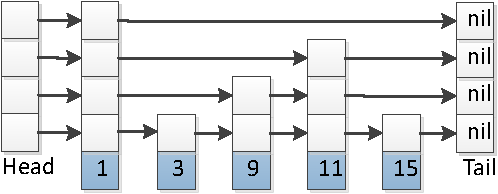
\includegraphics[width=0.5\textwidth]{img/skiplist-crop.pdf}
  \caption{A Skiplist representation of $\bf \{1,3,9,11,15\}$. The levels of
each node, respectively, are 3, 0, 1, 2, and 0.}
  \label{fig:skiplist}
\end{figure}

\subsection{Core Operations}

We now outline a few operations on Skiplists. In general, these are
quite similar to their linked-list counterparts. In fact, each Skiplist
operation can be decomposed into a sequence of linked-list operations that
each affect
one level of the Skiplist.

Suppose we want to search for element $e$. First,
we look at the list at $L(M)$ and traverse it linearly until we encounter
an element greater or equal to $e$.  If we encounter $e$, then we stop.
If we found an element greater than $e$, we repeat this procedure from
this new starting point. If we only encountered the tail of the list, then we
repeat the procedure starting from the first element in $L(M-1)$. This procedure
repeats until we successfully locate $e$. If we encounter either an element
greater than $e$ or end of the list at $L(0)$ we conclude $e$ is
not contained in the Skiplist. See Figs. \ref{fig:skiplist:search3} and \ref{fig:skiplist:search15}
for sample search runs on the Skiplist presented in Fig. \ref{fig:skiplist}.

To insert an element $e$ into a Skiplist, we first perform a search for the element
as previously described. However, we also keep track of additional information.
The insertion point is determined by where we stop searching at $L(0)$. Throughout the
search process, an array
$\texttt{previous}[i]$ is maintained that contains all the right-most pointers (at level $i$)
to elements left of the insertion point. An array $\texttt{next}[i]$ is given the previous values
of each pointer in $\texttt{previous}[i]$. To insert $e$, we assign it a random level $l$, set 
all the right-most pointers in $\texttt{previous}[i]$ for $0 \leq i \leq l$ to $e$ and set
the pointers emanating from $e$ to $\texttt{next}[i]$ for $0 \leq i \leq l$. Insertion has
the visual effect of simply splicing $e$ into the Skiplist (see Fig. \ref{fig:skiplist:insert5}.)

To delete an element $e$ from a Skiplist, we first search for the element (as we did for insertion).
If the element is not found, we are done. Otherwise, we should map each pointer in $\texttt{previous}[i]$
to the value in $\texttt{next}[i]$ for $0 \leq i \leq l$, where $l$ is the level of $e$. See Fig. \ref{fig:skiplist:insert5} for an illustration of deleting an element from a Skiplist.

\subsection{Additional Operations}
Pugh has defined \cite{pugh90a} a number of useful
operations such as merging Skiplists, splitting Skiplists, and
concatenating two Skiplists together when all the keys in one Skiplist
are less than or equal to the smallest key in a second Skiplist. However,
an operation that decreases the value of an element in a Skiplist (besides
simply deleting the old value and reinserting the decreased value) was not present and
we were unable to find a description of this operation in the literature.

\begin{figure}[H]
  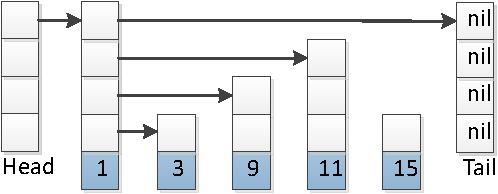
\includegraphics[width=0.5\textwidth]{img/skiplistSearch-crop.pdf}
  \caption{Skiplist traversal for finding the element 3 in the Skiplist presented in Fig. \ref{fig:skiplist}}
  \label{fig:skiplist:search3}
\end{figure}

\begin{figure}[H]
  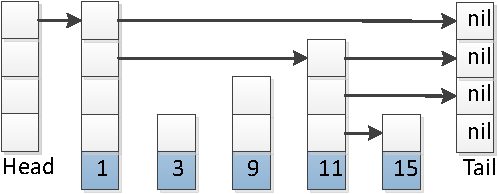
\includegraphics[width=0.5\textwidth]{img/skiplistSearch15-crop.pdf}
  \caption{Skiplist traversal for finding the element 15 in the Skiplist presented in Fig. \ref{fig:skiplist}}
  \label{fig:skiplist:search15}
\end{figure}

\begin{figure}[H]
  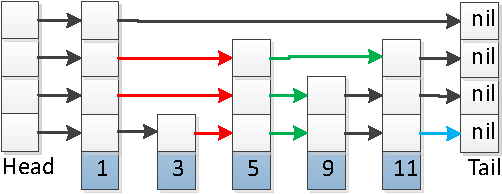
\includegraphics[width=0.5\textwidth]{img/skiplistInsert5-crop.pdf}
  \caption{Illustration of insertion and removal. 5 has been inserted into the Skiplist. Red indicates pointers contained in $\texttt{previous}[i]$, and green indicates pointers contained in $\texttt{next}[i]$. 15 has also been removed from the Skiplist and updated pointers for this operation are in blue.}
  \label{fig:skiplist:insert5}
\end{figure}

\subsection{Lock-Free Skiplists}
Shavit and Lotan's Skipqueue \cite{shavit00} is a modification
of Pugh's Skiplist that gives its operations lock-free guarantees.
We present a high-level technical summary of their work.
% and in
%Section \ref{skipqueue:decreasekey} we will
%build a \texttt{decreaseKey} operator for Skiplists using their approach.
Following with our analogy of Skiplist
operations being composed of operations on the linked lists formed at each level
of the Skiplist, we see that lock-free
operations on Skiplists can be composed of operations on lock-free linked lists.

One subtle issue with Shavit and Lotan's modifications is that $L(i)$ is not necessarily a subset
of all $L(k)$ (for $k < l$): a value's membership is determined by it being
in the lowest level of the Skiplist.
In particular, this means that even if we encounter
a target value in a higher level of the Skiplist, we still must verify it is
linked to the structure in $L(0)$. 

The search, add, and delete operations of a lock-free Skiplist follow the same form as
those we defined on Pugh's Skiplist.
However, here we need to handle the possibility of threads
concurrently modifying the Skiplist. To detect concurrent operations, we
modify our linked list's node datatype from the 2-tuple (\texttt{value}, \texttt{nextPtr[]}) to
the 3-tuple $(\texttt{value}, \allowbreak \langle \texttt{bool}, \allowbreak \texttt{nextPtr} \rangle\texttt{[]}$),
where \texttt{nextPtr} is the datatype used for pointers, and $\langle \texttt{bool}, \allowbreak \texttt{nextPtr} \rangle$
are written / read in a single atomic operation. In Java, this can be implemented
with the \texttt{AtomicMarkableReference} class.
In C/C++, this can be easily implemented by stealing a bit from a word-aligned pointer.
The boolean value serves as a deletion bit that is set whenever a node is removed
from the Skiplist but has yet to be physically removed from the linked list structure. This is
important for avoiding certain interleavings of operations. Consider two threads concurrently accessing
a Skiplist. The first thread reads the deletion mark on an element $a$ at level $i$, and is
interrupted by a second thread which marks the element as deleted. When the first thread resumes,
it will still assume that $a$ is not marked and, if inserting a new element,
could create an untraversable section of the
Skiplist by building on $a$'s next pointer.

To search for an element in a lock-free Skiplist we take the same approach as before, but
we additionally remove any marked nodes from the linked list structure and we always traverse
down to $L(0)$ in order to verify membership. To add an element
into the lock-free Skiplist we construct the \texttt{previous[i]} and \texttt{next[i]} sets
as before and set the next pointers of the new node to \texttt{next[i]}. We also update the
pointers in \texttt{previous[i]} to point to our new node (from level $0$ to level $l$).
If we are unsuccessful at having \texttt{previous[0]} point to our new node, we restart the
whole procedure since either a new node was inserted and the ordering of $L(0)$ may be violated
if we insert or the node at \texttt{previous[0]} was marked for removal.
Note that the linearization point of an add occurs when the element is inserted
into $L(0)$. Once \texttt{previous[0]} is updated, we attempt to update the remaining
\texttt{previous[i]} to \texttt{next[i]} in a CAS loop. To handle concurrent changes
during this process (e.g., \texttt{previous[i]} being marked), we recompute the \texttt{previous}
and \texttt{next} arrays whenever an atomic update fails.

Removing an element from a lock-free Skiplist is analogous to adding an element.
First, we search for the target element and compute our \texttt{previous[i]} and \texttt{next[i]}
arrays. Next, we mark each
\texttt{next} pointer of the target element in a top-down fashion within a CAS loop. When a CAS fails,
we re-read the relevant \texttt{next[i]} as another thread could have modified it (e.g., a
new node was linked to the node we're currently deleting.) When the \texttt{next}
pointer has been marked in $L(0)$, we consider the element removed (this is our linearization
point.) There is no need update any pointers on a removal since subsequent searches will perform
this for us.

%\subsection{A decreaseKey operator for Skipqueues}
%\label{skipqueue:decreasekey}
%Keeping track of the \texttt{next[i]} and \texttt{previous[i]}
%``windows'' of an element in a Skipqueue leads to a natural implementation
%of a \texttt{decreaseKey} operator where we re-use information from
%the deletion call. Suppose we have located the target element in the
%Skipqueue and it has a level of $j$. Let $i^*$ denote the index of the largest value
%in the \texttt{next} array that is smaller than the new value of the target. We can use
%$\mathtt{next[i}^*\mathtt{]}$ as the starting location for determining a new location
%for the decreased value of our target (since every node after $\mathtt{next[i}^*\mathtt{]}$
%is greater than our new value.) Aside from the head of the list, the insert is performed
%the same as before. If the attempt to insert needs to be restarted, we restart as a non-optimized insertion.

%The level of the decreased element is bounded above by $j$. On the first (the optimized) insertion attempt we
%set the level of the decreased element equal to $j$. This avoids introducing bias into the Skipqueue structure: if we sampled
%the new height from the discrete uniform distribution $U(0, j)$ we would force elements to gradually
%lose levels. If the optimized insertion attempt fails, there is no restriction placed on the level of the element.

\section{Pairing Heaps}
\label{sec:pheap}

Pairing heaps were developed by Fredman et al. \cite{fredman86} as
a simpler alternative to Fibonacci heaps that, at least empirically,
do not sacrifice performance.
Pairing heaps are a popular backing data structure
for Dijkstra's algorithm due to its offering of an efficient
\texttt{decreaseKey} and its avoidance of complicated tree rebalances.

% http://www.cise.ufl.edu/~sahni/dsaaj/enrich/c13/pairing.htm is good!

\subsection{Operations on Pairing Heaps}

We provide a sketch of the salient features of pairing heaps.
The main operator defined on pairing heaps is \texttt{meld}, which
accepts two heaps and uses a compare-and-link approach to join
its inputs together. See Fig. \ref{fig:meld} for an example of
melding two heaps together. The roots are compared and the root with the
largest value (assuming we have min-heaps) is added as the left-most
child of the smaller root. Insertion of a node is performed
by constructing a trivial heap containing only the relevant node
and melding it the main heap.

The supported pairing heap operations are as follows:
\begin{itemize}\addtolength{\itemsep}{-1\baselineskip}
\item[] $\mathtt{makeHeap}(h)$\\
\item[] $\mathtt{findMin}(h)$\\
\item[] $\mathtt{insert}(x, h)$\\
\item[] $\mathtt{deleteMin}(h)$\\
\item[] $\mathtt{meld}(h, h')$\\
\item[] $\mathtt{decreaseKey}(\Delta,x,h)$\\
\item[] $\mathtt{delete}(x,h)$\\
\end{itemize}
where $h,h'$ are pairing heaps, $x$ is a target node (or, equivalently,
a target value), and $\Delta > 0$ is the value by which the
target node should be decremented.

\begin{figure}
  \Tree [.3 [.5 \qroof{T_1}.10 [.12 \qroof{T_2}.19 \qroof{T_3}.20 ] \qroof{T_4}.34 ] !{\qframesubtree} [.25 [.19 \qroof{T_5}.20 \qroof{T_6}.21 ] \qroof{T_7}.42 ] ]
  \caption{Melding two min-heaps together (one with root 3 and the other with root 5) with the \texttt{meld} operator. The heap rooted at 5 becomes a subheap of the heap rooted at 3.}
  \label{fig:meld}
\end{figure}

\texttt{deleteMin} removes the minimum (root) element of a pairing heap $H$. Say once the root of the tree is removed we have $n$ sub-trees $H_1, H_2, \dots, H_n$, each with their own individual roots.
For each tuple in the set $\{(H_1, H_2), (H_3, H_4), \dots, \allowbreak (H_{n-1}, H_n)\}$, we meld the two heaps together to form $\{H'_1, \dots, \allowbreak H'_m\}$. It is worth mentioning that this pattern of
grouping into tuples (pairs) is where pairing heaps derive their namesake.
If $n$ is odd, $H_n=H'_m$ is not melded.
Finally, we perform a right-iteration
(similar to foldr) of \texttt{meld} over these $m=\frac{n}{2}$ (or $m=\frac{n-1}{2} + 1$) heaps to construct a newly rebalanced pairing heap $H'$:
\begin{equation*}
  H' = \mathtt{meld}(H'_1, \mathtt{meld}(H'_2, \dots \mathtt{meld}(H'_{m-1}, H'_m) \dots ))
\end{equation*}
To make the ordering $H_1, H_2, \dots, H_n$ unambiguous, we say that $i^\mathrm{th}$ child of $H$ (i.e., the root of $H_i$) is the $i^\mathrm{th}$
most recently melded node to the root.
Note here that \texttt{deleteMin} rebalances the tree structure of the pairing heap. See Fig. \ref{fig:deletemin} for an illustration of calling
\texttt{deleteMin} on a Pairing heap.

\begin{figure}
  \begin{enumerate}
   \item[(a)] \Tree [.7 [20 15 8 9 42 ] ] 
   \item[(b)] \Tree [20 15 8 9 42 ]
   \item[(c)] \Tree [.15 20 ]
              \Tree [.8 9 ]
              \Tree [.42 ]
   \item[(d)] \Tree [.15 20 ]
              \Tree [.8 42 9 ]
   \item[(e)] \Tree [.8 [.15 20 ] 42 9 ]
  \end{enumerate}
  \caption{Calling \texttt{deleteMin} on a Pairing heap (a). The root is removed (b) and the children are melded in pairs (c), and then the pairs themselves are melded in right-to-left order (d-e). Note that the resulting heap (e) is more balanced than (a).}
  \label{fig:deletemin}
\end{figure}

\texttt{decreaseKey} is implemented as follows. Suppose
a node $x$ has its value decreased and this new value
violates the heap invariant (i.e., $x$ is now
smaller than its parent.) The subtree rooted
at $x$ is removed from the tree and melded
to the parent tree as previously described.

$\mathtt{delete}(x,h)$ is implemented by delinking the sub-tree $S$ rooted at $x$ from $h$, calling $\mathtt{deleteMin}$ on $S$, and melding the resultant
tree back to $h$.

%\texttt{removeRoot} is implemented in a novel way.
%First, a left-to-right pass is performed
%over the root's children. The children
%are grouped into pairs (this is where
%pairing heaps derive their namesake)
%and the largest child of each pair
%is made a child of the smallest. Next,
%a right-to-left pass is performed over
%the grouped trees and they are merged
%together.

\section{Parallelizing Dijkstra's Algorithm}
\label{sec:dijkstra}
We now consider some issues pertinent to parallelizing a heap-backed
implementation of Dijkstra's algorithm. If \\ \texttt{deleteMin} does not
remove and return the unvisited node in the graph with the smallest distance
from the source node, Dijkstra's algorithm is not guaranteed to solve the shortest-path problem.
A na\"{i}ve approach to running Dijkstra's algorithm in parallel would be to allow calls
to \texttt{deleteMin} and \texttt{decreaseKey} haphazardly interleave. However,
the minimum of the heap will change on some call to \texttt{decreaseKey} if
a new value of a node is less than the current value. Thus, some comparison
is needed to see if calls to \texttt{decreaseKey} will produce a new minimum
value in the heap. There are three basic approaches to solving this problem:

\begin{enumerate}
  \item Optimistically continue removing minimum elements from the heap. 
  \item Pessimistically check if any of the new distances are less than the minimum of the heap, and continue
    if the minimum will remain unchanged. This has an advantage over the next method where the decision to continue
    can be made without any modifications to the heap.
  \item Pessimistically assume that \texttt{decreaseKey} will always produce a new minimum and ensure that
    all calls to \texttt{decreaseKey} complete before the next iteration's call to \texttt{deleteMin} executes.
\end{enumerate}

Solution 1 requires complicated interactions between concurrent states of the heap
or requires independent copies of the heap to be made and later merged. Since there are
two choices for every iteration of Dijkstra's algorithm (either the heap's minimum changes
or does not change), a copying approach requires $\mathcal{O}(2^n)$ copies to be made, which is
intractable for large graphs.

Solutions 2 and 3 are both practical. We opt for solution 3 since it is simpler, but
for future work we may consider solution 2.

\section{Lock-Free Pairing Heaps}
\label{sec:ph}

In this section we develop lock-free \texttt{insert} and \texttt{decreaseKey}
operators for Fredman et al.'s pairing heap. Our
work relies on the observation that
the specifics of
Dijkstra's algorithm allow us to make assumptions about how
Pairing heap operations interleave. 
We first list some assumptions that we have made about overlapping
calls to operations on the heap and give a high-level overview
of our lock-free approach. In section \ref{sec:ph:roadblocks}
we give a technical overview of the difficulties encountered
in developing a lock-free Pairing heap and give a high-level
outline of our solutions to these issues.
In section \ref{sec:ph:ops} we delve into the details of our
\texttt{insert} and \texttt{decreaseKey} operators, in \ref{sec:ph:linear} we show
our operations are linearizable and discuss the semantics
of our lock-free pairing heap, and in \ref{sec:ph:correct} we sketch and informal proof
regarding the correctness
of our implementation.

In section \ref{sec:dijkstra} we analyzed the specific performance bottle-necks and other
issues with running Dijkstra's algorithm in parallel. In particular, we noted that the
linearization guarantees provided by presently available concurrent heaps are insufficient for
blindly executing
concurrent calls to \texttt{deleteMin} and \texttt{decreaseKey}. Hence, we assume
these calls will never interleave, and, further, that only concurrent calls to 
\texttt{decreaseKey} overlap.

\subsection{Developmental Roadblocks}
\label{sec:ph:roadblocks}

There are a number of issues that must be overcome when developing
a lock-free Pairing heap. A design problem pertinent to all lock-free data
structures is how to efficiently broadcast when one thread has made modifications
that possibly interfere with concurrent work \cite{herlihy91}. 
For a Pairing heap, we have identified
four such coordination problems that arise from the need to
maintain the heap root, the parent of a node in the heap, and
the children of a heap node.

The first roadblock is that Pairing heap operations contend to
make changes to the root of the heap when a node is produced (either a newly inserted
node or an existing node that has sufficiently decreased)
that is lower than all values currently in the heap.
Nodes could be incorrectly deleted if \texttt{insert} and \texttt{decreaseKey}
were to override the root of the heap without consideration of other changes.
For example, if we concurrently \texttt{insert} two new values $a,b$ (where $a < b$) into a
heap that are both lower than all existing heap values, the intended state of the heap
has $a$ at the root, $b$ as its child, and the remainder of the heap a child of either $a$
or $b$. If
$a$'s insertion linearizes before $b$'s insertion, the call to insert $b$ must detect this
and instead change its strategy to inserting $b$ as a child of $a$. We have resolved
this issue by using a \texttt{CAS}-loop that only commits changes to the heap root
if no other changes have been made.

Another roadblock in designing a concurrent Pairing heap is that calls to
\texttt{decreaseKey} and \texttt{insert} that produce new roots
compete to change the parent of the current root. Continuing along the same
lines as our previous example, suppose that while inserting $a$ and $b$,
$a$ linearizes first and hence has the old root as its child. If $b$ concurrently
tries to insert itself as the root, it will fail by the detection protocol established
in the previous paragraph, but not before changing the root's parent from $a$ to $b$.
We resolve this problem by duplicating the old root of the heap and updating
the parent field of the clone. This yields a useful property:
if the new root fails to be \texttt{CAS}ed into place, no other node has
access to the cloned previous root and it can safely be discarded.

However, we have
introduced an additional problem: when the new root has been inserted, references
to the old root must be atomically updated to the newly cloned node. In particular, this
presents difficulties when maintaining references
to nodes outside of the pairing heap structure. (For example, if an adjacency list
of Pairing heap nodes is used in a graph, references must be updated.)
We resolve this issue by first introducing an additional layer of indirection: all references
to a Pairing heap node are made through a common reference object (pointer.) And, secondly,
we ensure the process of updating the new location occurs atomically by the using
a Descriptor-based design (see \cite{fraser07} and \cite{dechev10}.) Descriptor objects
combine the global state of an object and instructions for carrying out an operation.
In our approach, Descriptors enclose the root node (the global state of the Pairing heap)
and updating the memory location of the previous root (a pending operation.)

Our final coordination issue is that calls to \texttt{deleteMin} and \texttt{insert}
also compete to insert nodes as a child of the current root. Say $r$ is the root
of the heap and we insert elements $a,b > r$. Both $a$ and $b$ will attempt
to insert themselves as the left-most-child of $r$. We solve this issue by storing
child nodes in a lock-free linked list (a Michael-Scott \cite{michael96} queue.)

\subsection{Lock-free insert and decreaseKey Operations}
\label{sec:ph:ops}

\begin{algorithm}
  \SetKwFunction{meld}{meld}
  \SetKwFunction{NewRootDescriptor}{NewRootDescriptor}
  \SetKwFunction{CAS}{CAS}
  \KwIn{A Pairing heap $H$ and new node $e$}
  \KwOut{$e$ will be added to $H$}
  \Begin{
    \While{true}{
    \tcp{Case $1$}
      Descriptor $d$ $\leftarrow$ $descriptor$.get()\;
      $d$.execute()\;

      \If{$e$.distance $\geq$ $d$.$root$.distance}{
        $e$.parent $\leftarrow$ $d$.$root$\;
        $d$.$root$.subHeaps.add($e$)\;
        break\;
      }

      \tcp{Case $2$}
      Node $rootClone$ $\leftarrow$ $d$.$root$.clone()\;
      $e$ $\leftarrow$ \meld{$rootClone$, $e$}\;
      Descriptor $dNew$ $\leftarrow$ \NewRootDescriptor{$e$, $d$.$root$, $rootClone$}\;

      \If{\CAS{$descriptor$, $d$, $dNew$}}{
         $descriptor$.get().execute()\;
         break\;
       }
       \Else{
         $e$.subHeaps.remove($d$.$root$)\;
         $descriptor$.get().execute()\;
       }
    }
  }
\caption{A lock-free \texttt{insert} operator for Pairing heaps.}
\label{alg:insert}
\end{algorithm}

\begin{algorithm}
  \SetKwFunction{meld}{meld}
  \SetKwFunction{NewRootDescriptor}{NewRootDescriptor}
  \SetKwFunction{UpdateRootDescriptor}{UpdateRootDescriptor}
  \SetKwFunction{CAS}{CAS}
  \KwIn{A Pairing heap $H$, a target node $key$, and a new weight $w$}
  \KwOut{$key$'s value in the heap will be decreased to $w$.}
  \Begin{
    \If{!$key$.inHeap || $key$.distance $\leq$ $w$}{
      return\;
    } 
    \tcp{Case $1$}
    \While{key == $descriptor$.get().root}{
      Descriptor $d$ $\leftarrow$ $descriptor$.get()\;
      $d$.execute()\;
      \If{$d$.root != key}{
        break\;
      }
      $newRoot$ $\leftarrow$ $key$.clone()\;
      $newRoot$.distance $\leftarrow$ $w$\;
      Descriptor $dNew$ = \UpdateRootDescriptor{$d$.root, $newRoot$}\;
      \If{\CAS{$descriptor$, $d$, $dNew$}}{
        $descriptor$.get().execute()\;
        return\;
      }
      \Else{
        $descriptor$.get().execute()\;
      }
    }
    
    \tcp{Case $2$}
    $descriptor$.get().execute()\;
    $key$ $\leftarrow$ $key$.getPointer().getNode()\;
    $key$.distance = $w$\;
    \If{$key$.parent.distance $\leq$ $key$.distance}{
      return\;
    }
    
    $key$.parent.subHeaps.remove($key$)\;
    
    \While{true}{
      \tcp{Case $3$}
      Descriptor $d$ $\leftarrow$ $descriptor$.get()\;
      $d$.execute()\;
      
      $key$ $\leftarrow$ $key$.getPointer().getNode()\;
      \If{$key$.distance $\geq$ $d$.$root$.distance}{
        $key$.parent $\leftarrow$ $d$.$root$\;
        $d$.$root$.subHeaps.add($key$)\;
        return\;
      }
      
      \tcp{Case $4$}
      $key$.parent $\leftarrow$ null\;
      Node $rootClone$ $\leftarrow$ $d$.$root$.clone()\;
      $key$ $\leftarrow$ \meld{$rootClone$, $key$}\;
      Descriptor $dNew$ $\leftarrow$ \NewRootDescriptor{$key$, $d$.$root$, $rootClone$}\;
      
      \If{\CAS{$descriptor$, $d$, $dNew$}}{
        $descriptor$.get().execute()\;
        break\;
      }
      \Else{
        $key$.subHeaps.remove($d$.$root$)\;
        $descriptor$.get().execute()\;
      }
    }
  }
  \caption{A lock-free \texttt{decreaseKey} operator for Pairing heaps.}
  \label{alg:decreaseKey}
\end{algorithm}

\begin{algorithm}
  \SetKwFunction{NewRootDescriptor}{NewRootDescriptor}
  \SetKwFunction{UpdateRootDescriptor}{UpdateRootDescriptor}
  \SetKwFunction{CAS}{CAS}
  \If{$d$.pending}{
    \CAS($d$.node, $d$.oldRoot, $d$.newRoot)\;
    $d$.pending = false\;
  }
  \caption{Execution of a \texttt{NewRootDescriptor} $d$.}
  \label{alg:newroot}
\end{algorithm}

\begin{algorithm}
  \SetKwFunction{NewRootDescriptor}{NewRootDescriptor}
  \SetKwFunction{UpdateRootDescriptor}{UpdateRootDescriptor}
  \SetKwFunction{CAS}{CAS}
  \If{$d$.pending}{
    \CAS($d$.root, $d$.oldRoot, $d$.newRoot)\;
    $d$.pending = false\;
  }
  \caption{Execution of a \texttt{UpdateRootDescriptor} $d$.}
  \label{alg:newroot}
\end{algorithm}

Our \texttt{insert} and \texttt{decreaseKey} operators utilize
a Descriptor-based design: threads race to place Descriptors that
describe operations to a Pairing heap. In general, our Descriptors
are fine-grained and encapsulate changes to only one or two memory addresses.

Our \texttt{insert} operation first processes any pending operations.
The insertion process is split into two cases. In the first case
(lines 5-9 in Algorithm \ref{alg:insert}), the value of the
root is less than or equal to the value of the node to be inserted,
and the node is insert as the left-most child of the root.

In the second case (lines 10-19), the new node's value is less than the 
the value of the root, and the root must be updated. To accomplish
this update, we create a NewRootDescriptor that contains the
new root, the old root, and the new memory address for the old root.
We then try to \texttt{CAS} this descriptor into place. If \texttt{CAS}
fails, we remove the root of the heap from the node we are inserting, process
the current descriptor (if applicable), and retry.

Our \texttt{decreaseKey} operator is broken into four cases.
In the first case (lines 5-21 of Algorithm \ref{alg:decreaseKey}),
we are decreasing the value of the current heap root. We first
execute any pending operations, copy the current root, decrease
the copy's value, and create a UpdateRootDescriptor that contains
the new root and the memory location of the root of the heap. We then try
to \texttt{CAS} the descriptor into place. If \texttt{CAS} succeeds,
we are done. Otherwise, we retry after processing the descriptor
if the target is still the root of the heap, or we move onto
another case if the root has changed.

In the second case (lines 22-27), the new value of the node is still less than or equal to
its parent's value. No structural changes to the heap are required in this case:
we handle this case by simply changing the value of the node. One of our assumptions
for \texttt{decreaseKey} is that calls to change a particular node do not
interleave. A key benefit from this assumption is that this second case can proceed
in a wait-free manner since no memory locations require an update.

Before executing the remaining two cases (lines 28-50), we remove the target node from its parent's
list of subheaps as both cases involve moving the node to a new location
in the heap. The final cases are largely identical to the cases of our \texttt{insert} operator
as we are essentially inserting a new node into the heap. In the third case
(lines 32-37), the node is larger than the current root and should be inserted
as a child of the root. In the fourth case (lines 38-49), the new value of the target
node is less than the value of the root and we insert the target node as the new
root of the heap.

\begin{figure}
  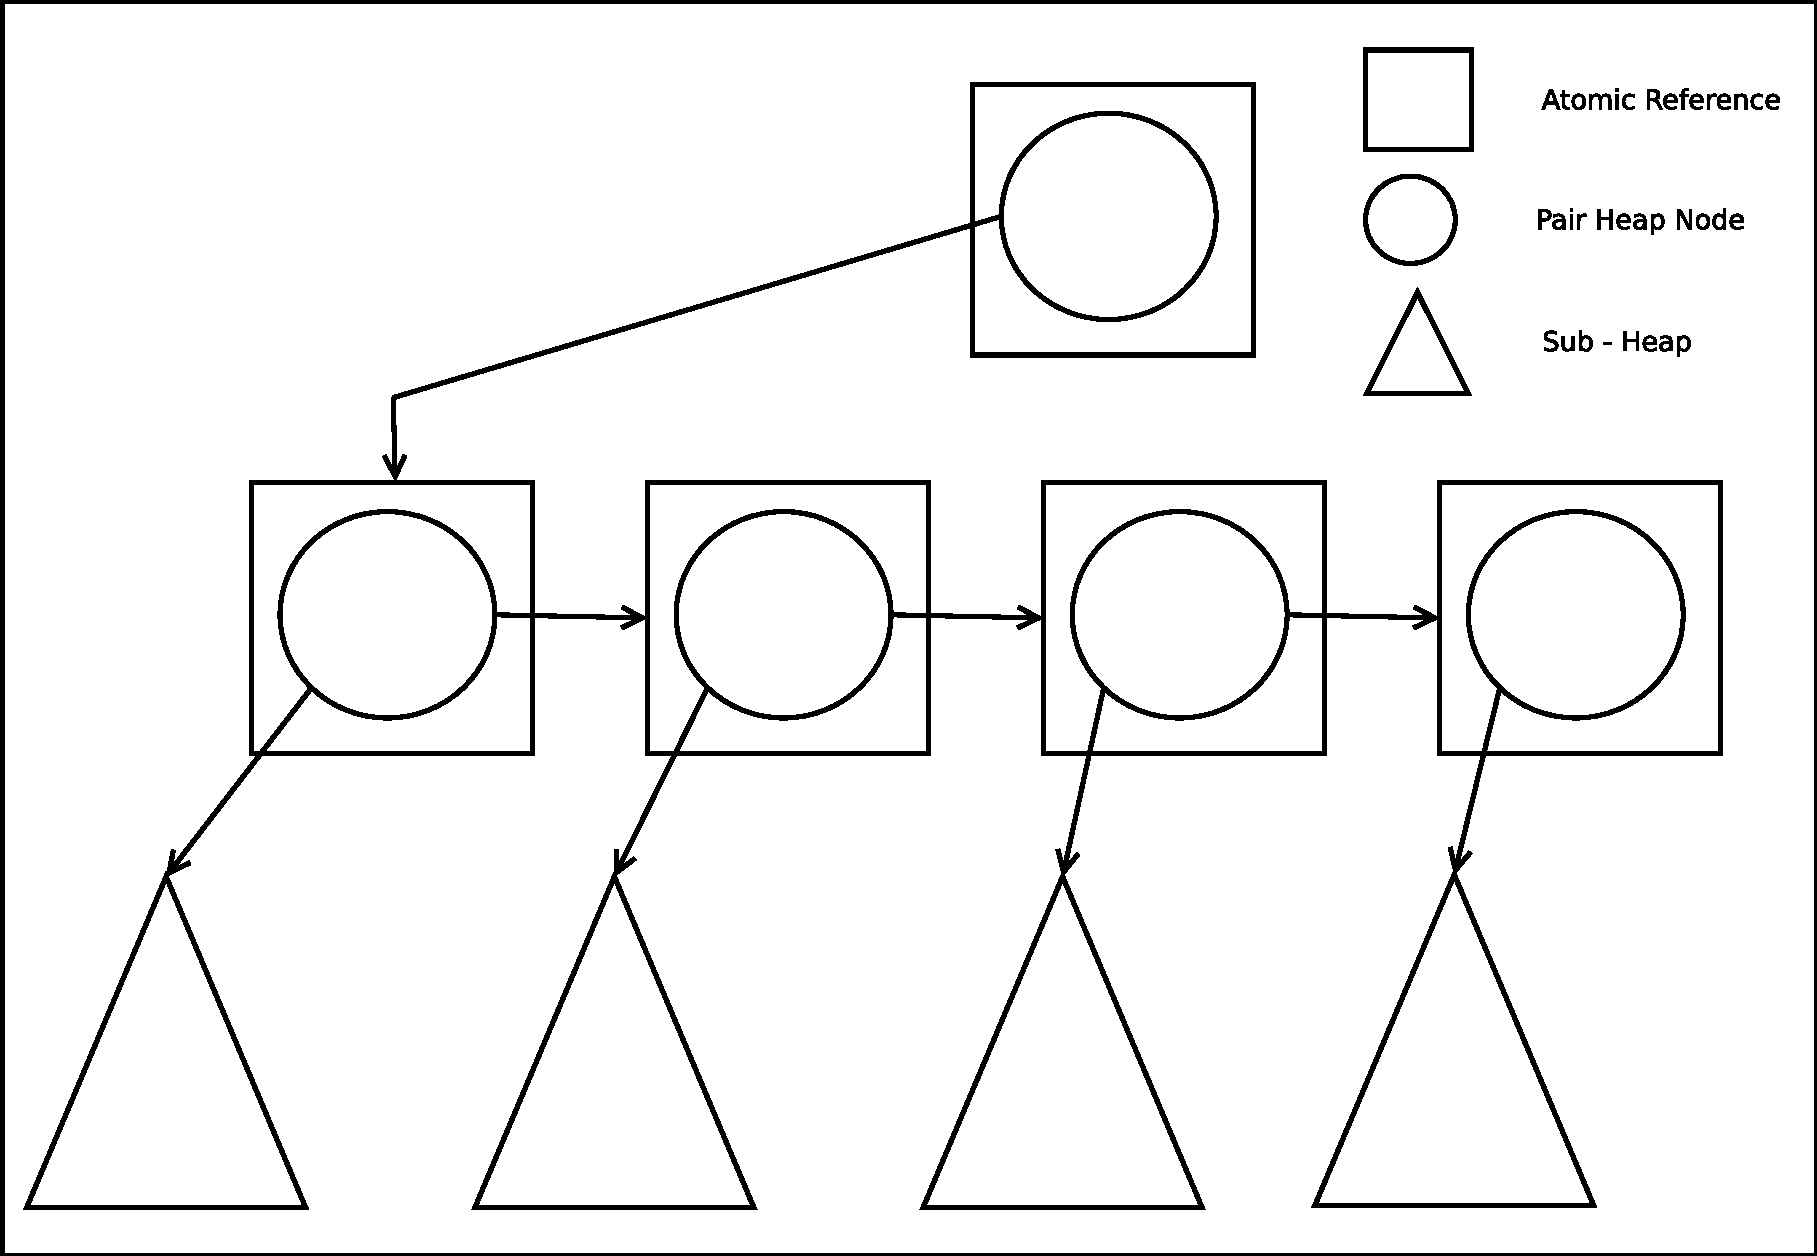
\includegraphics[width=0.45\textwidth]{img/PairHeapConcurrent-crop.pdf}
  \caption{Illustration of the concurrent pair heap structure. Pair heap nodes exist inside atomic references and hold atomic references to other heap nodes.}
  \label{fig:pairheap:structure}
\end{figure}

\subsection{Linearization Points}
\label{sec:ph:linear}
In this section we discuss the semantics of our lock-free Pairing heap and
its linearization points. An operation is linearizable \cite{herlihy90} if
it atomically takes effect at some time $t$ between the operation's invocation and its
response. In our Pairing heap implementation, an operation linearizes when
its changes to the heap take place.

Suppose we have $n$ operations $\{\sigma_1, \dots, \sigma_n\}$, each either a
call to \texttt{insert} or \texttt{decreaseKey}, concurrently executing. Let
$t_{desc}^i$ and $t_{op}^i$ denote the time instants at which, respectively, $\sigma_i$
atomically updates the Pairing heap's global descriptor object and when the memory writes
encapsulated by $\sigma_i$'s descriptor object are executed. Note that a descriptor placed
by $\sigma_i$ may be executed by $\sigma_i$, some $\sigma_j$ (where $j \not= i$),
or completed by many $\sigma_j$'s each performing partial work on the descriptor. Also,
let $t_s^i$ denote the time where any changes to the list of subheaps of a particular
node is modified by the operation $\sigma_i$.

We now turn to discussing the linearization points for an \texttt{insert} operation:
an \texttt{insert} that involves placing the new node as a child of the current root
linearizes at $t_s^i$
when it is successfully placed into the list of subheaps (line 7 of Algorithm \ref{alg:insert}.)
An \texttt{insert} that causes a root to be updated linearizes when its descriptor
is placed at $t_{desc}^i$ (line 13.) In both of these cases, the structure of the resultant heap
was determined when the global descriptor was read at line 3.

As previously discussed, the final two cases for our \texttt{decreaseKey} operator
are semantically identical to the two cases for \texttt{insert}. Hence, the
linearization points for these two cases also align. By the same reasoning discussed
in the previous paragraph, a \texttt{decreaseKey} operation falling into
case three (lines 32-37 of Algorithm \ref{alg:decreaseKey}) linearizes at $t_s^i$ (line 35),
and an operation falling into case four linearizes at $t_{desc}^i$ (line 42.) The heap's structure
is determined by the particular descriptor read at line 30.

For the first case of \texttt{decreaseKey} (where we decrease the root of the heap), the operation
linearizes when we place the descriptor into memory at $t_{desc}^i$ (line 14)
and the heap structure is determined
at line 6. For the second case of \texttt{decreaseKey} (where the new value of the node is still
greater than the parent and no structural changes are needed), the linearization point occurs
when the value of the node is changed at line 24.

\subsection{Correctness}
\label{sec:ph:correct}
In this section we discuss how our concurrent
operations on Pairing heaps in all cases maintain the heap invariant
and preserve the serial semantics
of the \texttt{insert} and \texttt{decreaseKey} operations on Pairing heaps.

For serial Pairing heaps, an \texttt{insert} has two effects on the
heap structure: either the new
node becomes the new root of the Pairing heap (and the old root becomes its child)
or the new node is added as the left-most child of the root of the Pairing heap.
A \texttt{decreaseKey} has three effects: either the new node becomes (or is already)
the heap root, is added as the left-most child of the first heap, or the target
node does not change location at all.

We show that for all interleaving cases of \texttt{insert} / \texttt{decreaseKey},
the resulting modifications to the Pairing heap are consistent with some
ordering of the same operations performed sequentially.
Note that we continue with our assumption that concurrent calls
to modify the same node in the heap do not occur. Note that both cases
of \texttt{insert} are equivalent to the final two cases
of \texttt{decreaseKey}, so we are free to omit discussion of \texttt{insert}.

\textbf{Case 1.} 
Suppose we are decreasing a root of the heap (lines 5-21 of Algorithm \ref{alg:decreaseKey}.)
If another thread is decreasing an older root, then the descriptor
has been modified and the CAS on line 14 will fail for that thread.
When the descriptor is re-read, the
current key will no longer be the root and the thread will be forced
to complete their operation in a new case. If another thread is decreasing its heap
to a value that is still less than its current parent (lines 23 - 27), then
this does not involve any structural changes to the heap. The root modification
can occur unaffected by this decrease. If the parent of the node being
decreased is the root, since the reference to the parent node is made through
a wrapper object (instead of a direct reference to the parent), the parent-child
relationship will be preserved even though the root node is located at a
new memory address (it is cloned, see line 11.)

The first interesting cases occur when we interleave a root update
with a \texttt{decreaseKey} call that
requires making changes near the root. Suppose a root update is interrupted by
a second thread falling into the third case (the newly decreased node is made
a child of the root.) However, no changes to the root are made in this case. The cloned
root and the original root that exist in the root update (line 11) both share a 
reference to the same list of subheaps. Hence, the addition of the node is
made immediately visible to both roots and successfully linearizes regardless of
if the root is changed or not. A peculiar edge case here is when the root
modification linearizes after the descriptor containing the old root
has been read (line 14 completes after line 30.) The decreased node will
be added on as a child of the old root, which is consistent with the Pairing heap state
obtained when the child node decrease linearizes before the root modification linearizes.
Otherwise, if the root modification linearizes before the descriptor has been read, the
newly decreased child node will be added with the new root as its parent.

If the decreased node is less than the current root, there is a race to update
the current root: either the decreased root will remain the root, or the newly
decreased node will become the root. The linearization point
for these cases is the CAS calls on lines 14 and 42, where the descriptor is updated.
There are a few different cases to consider here. Let $r$ and $r'$ respectively
denote the old and new values of the root (note $r' < r$) and say $n$ is the 
new value of the node to be decreased. Since we are in lines 38-49, 
we additionally have $n < r$. Say that $r' < n < r$. If the new value of the
root linearizes before the decreased node linearizes (if line 14 executes
before line 42), then $n$ will be the left-most child of $r'$. Otherwise,
if the decreased node linearizes before the root, the CAS on line 14 will
fail, and the root update will continue on to case 4. Next, suppose
$n < r' < r$. If the newly decreased node $n$ becomes the root
before $r'$, then $r'$ will be the left-child of $n$ and the CAS
on line 14 will fail. Since $n < r'$, $r'$ will insert as a node in case 2.
Note that executing the descriptor on line 22 ensures that the old root's
memory address is updated before we decrease its value on line 24. Otherwise,
if the root's value changes to $r'$ before $n$ becomes the root, then the CAS
on line 42 will fail and the descriptor to perform the memory address
update from $r \rightarrow r'$ will be performed at line 31 (if it was
not executed already by some competing thread.) Since $n < r'$,
the node decrease will remain in case 4.

\textbf{Case 2.} 
Next we consider situations where
operations (other than case 1 operations, which we have
already considered) interleave with case 2 of \texttt{decreaseKey} (lines 22-27 of Algorithm
\ref{alg:decreaseKey}.) Note that two competing case 2 operations on the same
node cannot interleave by our assumption that no two calls to decrease the
same node interleave. Also, if two case 2 operations interleave on
non-connected parts of the heap, they clearly cannot interfere with
each other. The case where we decrease a parent $P$ with value $p$ to $p' < p$
and a child $C$ of $P$ to $c' < c$ requires no structural changes. The linearization
point for these interleavings when the value of the node is updated at line 24.
The child node only proceeds to case 2 if $p \leq c'$ (if $P$'s change has not yet
linearized) or of $p' \leq c'$ (if $P$'s change has linearized.) However, since $p' < p$
and $p \leq c'$ we have $p' < p \leq c'$ and $C$'s new value is a valid child of
both $p'$ and $p$. Hence, we can proceed without making any structural changes to the heap
for these interleavings.

If a case 2 (lines 22-27) modification interleaves with
a root modification (cases 3 and 4, lines 30-37 and lines 38-49),
there are no possible concerns if we are modifying a node that
is not $P$ (adopting the same notation as before.) Further, if
$P$ is being modified in cases 3 or 4 while its child $C$ is being
modified in case 2, then the $C$ is certainly still a valid
child of $P$ for the same reason, namely that $P$'s value will only decrease.

\textbf{Case 3.} 
We now consider interleavings with case three (lines 30-27 of Algorithm
\ref{alg:decreaseKey}.) We have already covered two interleavings (cases 3 and 1
and cases 3 and 2.) If two concurrent calls to \texttt{decreaseKey}
both fall into the third case, both will race to be the left-most child
of the current root. The linearization point here is inside the \texttt{add}
method of the Michael-Scott \cite{michael96} linked-list based queue.
The Pairing heap state (i.e., the ordering of the children) is consistent with the order
in which these nodes reach this linearization point. If the fourth case
executes concurrently with the third case, then there is a question about
whether the node being decreased in the third case becomes a child of
the old root or the new root. The descriptor read on line 30 contains
the current root of the heap, and this determines which of the potential
roots becomes the parent of the node being decreased. Note that even
if the root changes between when the descriptor is read and when
the node becomes a child of the root, the target node becomes a child
of the node contained in the descriptor. Hence, the modifications
to the Pairing heap state that result from the interleavings of cases 3
and 4 are always consistent with the moment in time the descriptor was read.

\textbf{Case 4.} 
Lastly, we consider the case where two newly decreased nodes are both
less than the current value of the root and each contend to be the new
root (case 4 - lines 22-27 of Algorithm \ref{alg:decreaseKey}). Suppose
the root has value $r$ and the newly decreased nodes have values $n$ and $m$
such that $n, m < r$. Without a loss of generality, we assume that $n < m$
(the proof is the same for $m < n$, but with their respective roles
reversed) The linearization point for case 4 is when the descriptor
is placed into memory using CAS (line 42.) Suppose that the node
with value $m$ places its descriptor first. Then, the node with
value $n$ will fail to insert its descriptor and retry. Since $n < m$,
the node with value $n$ will again fall into case 4 and retry inserting
its descriptor. When this succeeds, $m$ will be its left-most child.
Alternatively, suppose $n$ inserts its descriptor first. Since $m > n$, 
$m$ will retry in the third case (lines 30-37). Finally,
we consider the case where $n = m$. Here, either node being
the new root is a valid state, and the winner is determined by whichever
node inserts its descriptor first on line 42. The remaining node will insert
itself as a child of the winner (i.e., case 3.)


Note that since case 4 (lines 38-49) clones the current root of the heap, if the CAS
call on line 42 fails, the old root is never modified and no other threads
have access to this cloned node. This prevents a race condition where one
thread overrides the parent field modification of another thread. Also
note that our assumption that no two calls to \texttt{decreaseKey} change
the same node ensures that the dangerous-looking changes to the
list of subheaps on lines 40 and 47 are safe. In particular, we are
certain to not, say, detach a node from a parent previously added by
another call to \texttt{decreaseKey}.


%In our concurrent Lock-free \texttt{insert} operator for Pairing heaps, the current root
%of the heap is read at line 3 (Algorithm \ref{alg:insert}) and the structure of the
%heap is determined from this point. If the root specified
%in the descriptor is smaller than the new node, the 

\section{Experimental Results}
\label{sec:exp}
In this section we compare the performance of lock-free Pairing heaps against
Shavit and Lotan's Skipqueues \cite{shavit00}, a priority queue based
on a lock-free implementation of Pugh's \cite{pugh90a} Skiplist.
We ran a concurrent version of Dijkstra's algorithm (outlined in 
\ref{sec:dijkstra}) that used Skipqueues and our lock-free Pairing heaps
and compared the search completion time.

The graphs experimented against were obtained from 
the Stanford Large Network Dataset Collection \cite{slndc}.
We considered two datasets: a graph of the citations made
between patents granted by the United States Patent and Trademark
Office (USPTO) \cite{leskovec05}
and a co-purchasing network graph from Amazon \cite{leskovec07}.

To produce these results, we selected a node whose degree
was equal to the mean degree of a vertex over the whole graph,
rounded up, if needed. This ensured we did not select a node
that biased our Pairing heap results due to its non-negligible 
start-up costs (see Section \ref{sec:exp:disc}.) For the amazon and patent graphs,
we searched on a varying number of threads ($1,2,4,8$), and
we report the average results obtained over $20$ and $8$ trials, respectively. 
Two machines were used for testing, one with an eight core i7 processor and another with an eight core Intel Xeon CPU           X5355 (2.66GHz). 

Results of the amazon and patent trials can be seen in Figure \ref{fig:ph:amazon} and Figure \ref{fig:ph:patent}.

The i7 machine outperformed the Xeon machine on all trials. 
There is a slight overall decrease in average runtime for the amazon dataset with the utilization of more threads. A similar decrease in average runtime can be seen in the US patent trials. 
If the longest runtime for $4$ threads in the i7 amazon trials is ommited, there is an increase in average runtime between $4$ and $8$ threads. The Xeon machine for the amazon data had an increased runtime for $4$ threads over $2$ threads and also $8$ threads over $4$ threads. For the use of $8$ threads, the runtime exceeded that of $1$ thread. Although average runtime decreases with the addition of threads in both trials, observed runtimes have high variance. Many runs with higher thread counts had higher runtimes than runs with less threads.


\begin{figure}[H]
  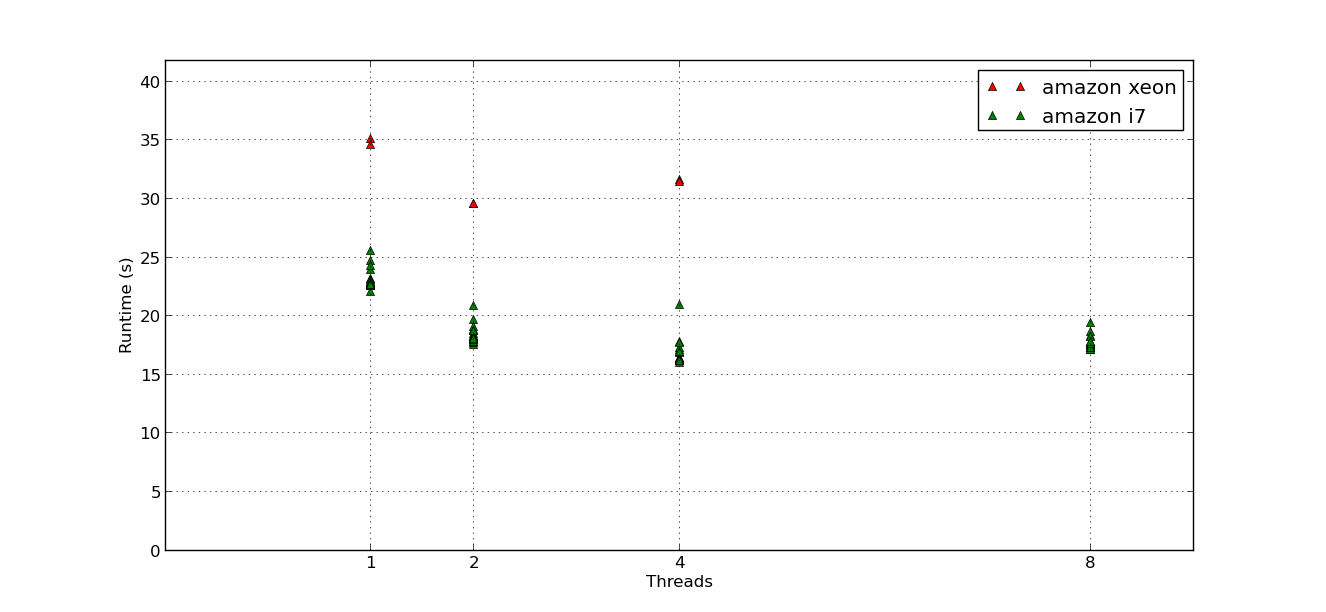
\includegraphics[width=0.45\textwidth]{img/amazon.png}
  \caption{Completion time of Dijkstra's algorithm on the Amazon co-purchasing database \cite{leskovec07}.}
  \label{fig:ph:patent}
\end{figure}

\begin{figure}[H]
  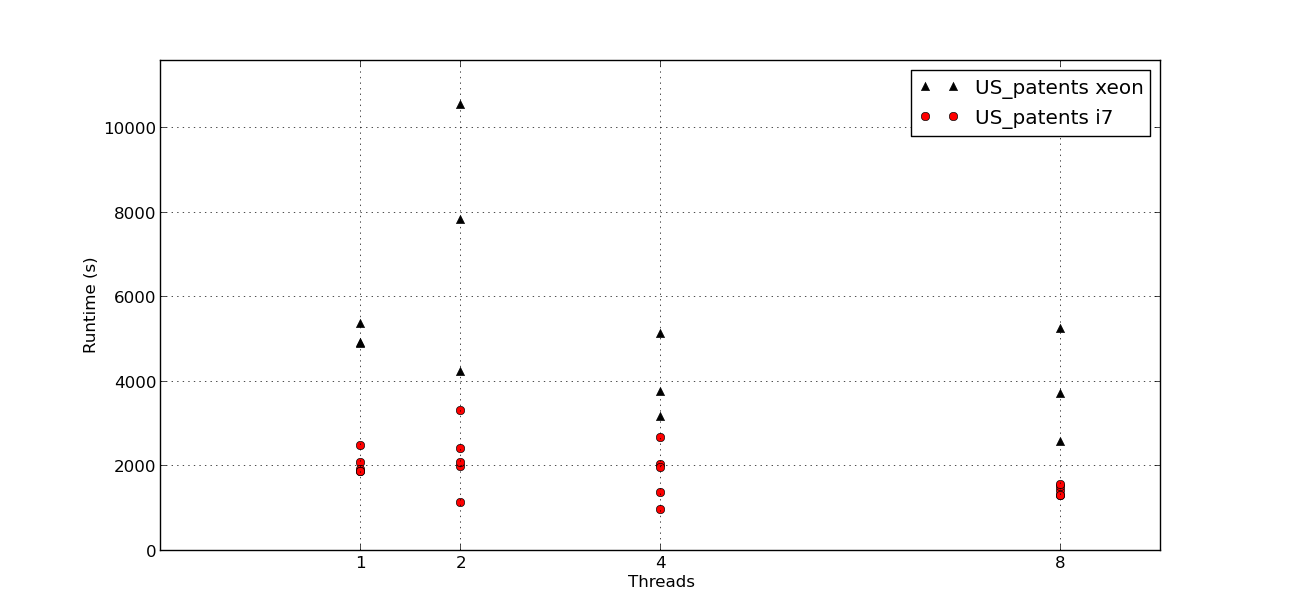
\includegraphics[width=0.45\textwidth]{img/US_patents.png}
  \caption{Completion time of Dijkstra's algorithm on the USPTO database \cite{leskovec05}.}
  \label{fig:ph:amazon}
\end{figure}


\section{Discussion}
\label{sec:exp:disc}
Our lock-free Pairing heap generally performed very poorly
when compared with a Skiplist-backed heap. We now turn
to discussing why this is the case and how this
can direct future improvements on our initial
algorithm design.

Consider the initial state of a Pairing heap constructed
to back a search for the shortest distances from vertex $v$
to all other vertices in the graph. The values in the heap
will initially (see Algorithm \ref{alg:dijk}) be $\mathrm{dist}(v) = 0$
and $\mathrm{dist}(u) = \infty$ for all other nodes $u \in \{u_1, u_2, \dots, u_n\}$.
This implies that
$v$ is the root of the heap and all other nodes $u$ are its children.
As each $u$ has an equal distance ($\infty$), there
is no real structure to the heap (see Figure \ref{fig:ph:start}.)

When we process the neighbors of $v$, we remove $v$ from the heap
as it is the minimum element. We replace it with some other unvisited
element (say $u_1$, see Figure \ref{fig:ph:start2}.) When we decrease
the distances of the neighbors of $v$, we delink them from their parents.
In our current implementation, each node stores its subheaps
in a Michael-Scott \cite{michael96} queue. Unfortunately, 
this data structure has a linear search time. If $|v|$ denotes
the degree of $v$, we have a total complexity of $\mathcal{O}(|v|^2)$, which
is not ideal. In a Pairing heap, this work is amortized over the life
of the data structure: early calls to \texttt{decreaseKey} occur in, at minimum, $\mathcal{O}(|v|)$
time, but later calls happen in near constant time. However, if $|v|$ is quite large, then
an unreasonable amount of time is spent performing the first \texttt{decreaseKey}.

\begin{figure}
  \Tree [.$v=0$ $u_1=\infty$ $u_2=\infty$ $\dots$ $u_n=\infty$ ]
  \caption{Start-up state of a Pairing heap backing Dijkstra's algorithm. The source node $v$ has a distance of $0$ and all other nodes $\{u_1,u_2,\dots,u_n\}$ are unvisited have currently have a of $\infty$.}
  \label{fig:ph:start}
\end{figure}

\begin{figure}
  \Tree [.$u_1=\infty$ $u_2=\infty$ $u_3=\infty$ $\dots$ $u_n=\infty$ ]
  \caption{State of a Pairing heap after running $\mathtt{deleteMin}()$ on the heap in Fig. \ref{fig:ph:start}.}
  \label{fig:ph:start2}
\end{figure}

%Efficiency of the lock-free Pairing heap will be examined by comparing the relative performance of Dijkstra's algorithm, backed by different heap structures, on large network data sets. Currently, we
%plan to test three variants of Dijkstra's algorithm. The first variant will backed by a normal Skipqueue that performs a \texttt{decreaseKey} by removing the target node and readding it with a decreased key value.
%The second variant will be backed with a Skipqueue that uses our optimized \texttt{decreaseKey} operator. The third variant will be backed with our lock-free pairing heap. We
%will use real world data sets collected from the Stanford Large Network Dataset Collection \cite{slndc} and Harvard's Human Interactome Database \cite{hid}. We will additionally use two
%synthetic graphs: a randomly generated dense graph and a randomly generated sparse graph.

%As pairing heaps are designed for efficiency in network applications such as shortest path finding, this is an ideal test case for this datastructure. Efficiency of parallel functionality will be examined for the data structure by determining runtime decrease by adding parallel functionality to the Dijkstra's implementation, through the use of the concurrent pairing heap.

%\section{Real-world performance of Lock-Free Pairing Heaps and Skipqueues}
We also observed a decrease in performance when the number of threads
working on \texttt{decreaseKey} operations were increased.
In blocking Pairing heaps, nodes are inserted (a similar procedure is used for \texttt{decreaseKey})
into the heap by either replacing the root of the heap or inserting itself as a subheap to the root.
A parallel variant Pairing heap variant that preserves the general form of insertion operations will place un-due contention near the root of the data structure.
Always inserting at the root appears to be a significant bottleneck.
Skipqueues, on the other hand, can insert elements in,
e.g., the middle of the list in a less-contended way
and are thus more parallel.

%However, insertions into a Pairing heap run in asymptotically less time than a comparable Skipqueue insertion: a Pairing heap
%insertion runs close to $\mathcal{O}(1)$ time but a Skipqueue insertion runs in $\mathcal{O}(\log n)$ time. This is due
%to the differing methods used to balance the heap structure.

\section{Future Work}
\label{sec:future}
In this section we
outline potential future directions for further research in developing efficient lock-free pairing heaps.

\subsection{Additional Operators}
We briefly outline a sketch of a parallelized \texttt{deleteMin} operator on Pairing heaps.
\texttt{deleteMin} follows what is essentially a Map-Reduce pattern: pairs of heaps are constructed
and then merged together to form a resultant heap. The first step has no contention between pairs
and is trivial to parallelize. Our \texttt{meld} operator can be used to merge heaps in parallel.

However, once a \texttt{deleteMin} process has started, the new heap root cannot be determined until
the call has finished.
To accomplish \texttt{deleteMin} in a lock-free manner, a Descriptor object could be placed into memory
that forces calls to other heap operations to first help complete the \texttt{deleteMin} before proceeding
to their own operations.

\subsection{Relieving Contention}
Our current implementations of \texttt{insert} and \texttt{decreaseKey} place
heavy contention on two memory addresses: the location containing the root of the heap
and the left child of the current root. The first contention arises from threads competing to
change the root of the heap, and the second from threads placing nodes under the root.
To prevent these contentious situations, an elimination strategy (similar to \cite{hendler04})
could be employed. As for two different node values $a,b$ either $a \leq b$ or $b < a$, two
contending nodes could be combined using the \texttt{meld} operator described in section \ref{sec:pheap}.
The greater of the two nodes would be added as a child of the lesser, and only the lesser would need
to contend for insertion near (or at) the root.

\subsection{Avoiding Large Start-up Costs}
A problem discussed in Section \ref{sec:exp:disc} is that
the initial state of the Pairing heap lends itself to
a $\mathcal{O}(|v'|)$ start-up time, where $|v'|$
denotes the number of edges connected to the source node.
There are two main ways to resolve this issue. First,
we could artificially introduce structure onto the initial heap state (see
Figure \ref{fig:ph:start3})
to reduce the search space for a particular node.
A second solution would be to replace the data structure that represents
the list of subheaps. For example, we could replace this with a Skiplist
(which offers $\mathcal{O}(\log n)$ search) or use a hash table to insert
search fingers \cite{hanson92} into our linked list.

\begin{figure}
  \Tree [.$v=0$ [.$u_1=\infty$ $u_2=\infty$ [.$u_3=\infty$ ] ] [.$u_4=\infty$ $u_5=\infty$ ] $\dots$ $u_n=\infty$ ] ]
  \caption{A more structured heap (see Figure \ref{fig:ph:start}.) Note that the heap invariant is not violated by a parent and child having equal weights.}
  \label{fig:ph:start3}
\end{figure}

\subsection{Profiling}

\section{Conclusion}


%\section{Lock-free Pairing Heaps}
%This section outlines our current thoughts about
%implementing a lock-free pairing heap.
%Lock-free procedures for pairing heaps will be implemented in a simlar manner to lock-free skip lists. The operat%ion delete min will require in depth analysis to avoid lock usage, as this method re-orders the entire heap. Other operations on the heap must remain active while a delete min operation is completing. A possible solution to this problem is to slightly loosen the restrictions on the heap properties. The loss of exactly following the pairing heap specification may lead to a lock-free solution while hopefully not compromising the integrity of the data structure.

%In
%\cite{shavit00} Shavit and Lotan construct
%a concurrent priority queue, coined a SkipQueue,
%based on Pugh's SkipList
%\cite{pugh90} data structure. We
%would like to adapt the principles outlined
%in \cite{fredman86} to Shavit SkipQueue.
%Specifically, we want to develop a corresponding
%\texttt{decreaseKey} operation on SkipQueues
%that allows an item in the heap to be
%decremented without the overhead of removing
%the item and adding a new item containing
%its decremented
%value.

%\section{Project Overview}

%This project will involve the following software
%development tasks:

%\begin{enumerate}
%  \item Develop a lock-based implementation of a pairing heap
%  \item Develop an implementation of Pugh's SkipLists
%  \item Develop an implementation of Shavit's SkipQueue.
%\end{enumerate}

%This project will involve the following research tasks:

%\begin{enumerate}
%  \item Propose an efficient \texttt{decreaseMin} operator for SkipQueues.
%  \item Determine if any additional optimizations can be made to enhance SkipQueues' performance
%    on the single-source shortest path problem.
%\end{enumerate}

%We will empirically evaluate the performance of a
%lock-based pairing heap, Shavit's SkipQueue, and
%our modified SkipQueue on a heap-backed version of Dijkstra's algorithm.
%We will test the performance of all these algorithms
%against the graph below with a varying number of threads.
%If we use C++ to implement lock-free pairing heaps we will use of the C++ pthreads library, as well as templates, to allow for the construction of a concurrent STL-like container class in C++. Further work may be explored by using the me%ssage passing interface (MPI).

%\begin{enumerate}
%\item A randomly-generated dense graph.
%\item A randomly-generated sparse graph.
%\item Graphs from Stanford's Large Network Dataset Collection \cite{slndc}
%\item Graphs from Harvard's Human Interactome Database \cite{hid}
%\end{enumerate}


% References
\bibliographystyle{abbrv}
\bibliography{proposal}

\end{document}
